\documentclass{article}
\usepackage{amsmath, amssymb, graphicx, verbatim, hyperref}

\title{\textbf{AMS595 Assignment 2} - Mandelbrot Set Boundary Approximation}
\author{Amol Arora, SBUID: 116491705} 
\date{\today}

\begin{document}
\maketitle

\section{GitHub Link}
\underline{All project files are uploaded here}:
\url{https://github.com/amol1202/AMS595_Assignment2}

\section{Introduction}
This project focuses on the Mandelbrot set, which is a set of complex numbers \( c \) for which the iteration of the function:
\[
z_{n+1} = z_n^2 + c
\]
remains bounded. For this project, we compute the boundary of the Mandelbrot set using numerical techniques, including:
\begin{itemize}
    \item A function to compute the divergence of a point \( c \) (whether \( z \) stays bounded or escapes).
    \item The bisection method to find the boundary of the Mandelbrot set.
    \item Polynomial fitting to approximate the curve.
    \item Numerical integration to calculate the length of the boundary.
    \item Visualization of the Mandelbrot set and its boundary.
\end{itemize}

\section{Methodology}
This section details the methods used to compute the boundary of the Mandelbrot set and approximate its length.

\subsection{Fractal Computation}
The Mandelbrot set is generated by repeatedly applying the function \( z_{n+1} = z_n^2 + c \), where \( z_0 = 0 \). If after many iterations, the absolute value of \( z \) grows larger than 2, the point \( c \) is considered to be outside the Mandelbrot set. We stop after 100 iterations and check whether \( |z| \) exceeds 2. If it does, the point is outside the set.

\subsubsection*{Fractal Function:}
The following code computes the number of iterations it takes for the point to diverge:
\begin{verbatim}
function it = fractal(c)
    z = 0;
    for it = 1:100
        z = z^2 + c;
        if abs(z) > 2.0
            return;
        end
    end
    it = 100; % Stays within the set
end
\end{verbatim}

\subsection{Bisection Method}
Once we have the fractal function, we need to find the boundary of the Mandelbrot set. We use the bisection method, a root-finding algorithm that splits the interval and finds where the function changes sign. We search along the imaginary axis for each real value \( x \) and apply the bisection method to find where the boundary occurs.

\subsubsection*{Bisection Method:}
\begin{verbatim}
function m = bisection(fn_f, s, e)
    tol = 1e-10;
    while abs(e - s) > tol
        m = (s + e) / 2;
        if fn_f(m) * fn_f(s) > 0
            s = m;
        else
            e = m;
        end
    end
end
\end{verbatim}

\subsection{Finding the Fractal Boundary}
We apply the bisection method along the real axis from \( x = -2 \) to \( x = 1 \), finding the boundary for each value of \( x \) by varying the imaginary part \( y \).

\subsubsection*{Boundary Detection Code:}
\begin{verbatim}
x_values = linspace(-2, 1, 1000);
y_boundary = zeros(size(x_values));

for i = 1:length(x_values)
    x = x_values(i);
    indicator_fn = @(y) (fractal(x + 1i * y) > 0) * 2 - 1;
    y_boundary(i) = bisection(indicator_fn, 0, 2); % Adjusted upper bound
end
\end{verbatim}

\subsection{Polynomial Fitting}
Once the boundary points are detected, we fit a 15th-degree polynomial to the boundary. This helps us represent the complex boundary as a smooth curve for further calculations.

\subsubsection*{Polynomial Fitting Code:}
\begin{verbatim}
valid_indices = (x_values > -1.8) & (x_values < 0.5);
x_fit = x_values(valid_indices);
y_fit = y_boundary(valid_indices);

p = polyfit(x_fit, y_fit, 15);

x_plot = linspace(min(x_fit), max(x_fit), 1000);
y_plot = polyval(p, x_plot);
\end{verbatim}

\subsection{Curve Length Calculation}
The length of the curve is computed using the formula for the arc length of a function:
\[
l = \int_a^b \sqrt{1 + \left(\frac{df}{dx}\right)^2} \, dx
\]
where \( f(x) \) is the polynomial representing the boundary.

\subsubsection*{Curve Length Calculation Code:}
\begin{verbatim}
function l = poly_len(p, s, e)
    dp = polyder(p);
    ds = @(x) sqrt(1 + polyval(dp, x).^2);
    l = integral(ds, s, e);
end

s = min(x_fit);
e = max(x_fit);
boundary_length = poly_len(p, s, e);
fprintf('Approximate length of the Mandelbrot set boundary: %.4f\n', boundary_length);
\end{verbatim}

\section{Results}
\subsection{Mandelbrot Set Visualization}
The Mandelbrot set was visualized by applying the \texttt{fractal} function over a grid of complex numbers. The result was a plot showing which points belong to the Mandelbrot set.

\begin{figure}[h!]
    \centering
    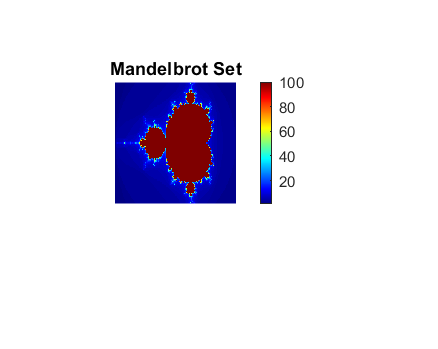
\includegraphics[width=0.5\textwidth]{mandelbrot_results/mandelbrot_set.png}
    \caption{Mandelbrot Set Visualization}
\end{figure}

\subsection{Boundary of the Mandelbrot Set}
The boundary points of the Mandelbrot set were computed using the bisection method. The boundary was then approximated by a polynomial fit.

\begin{figure}[h!]
    \centering
    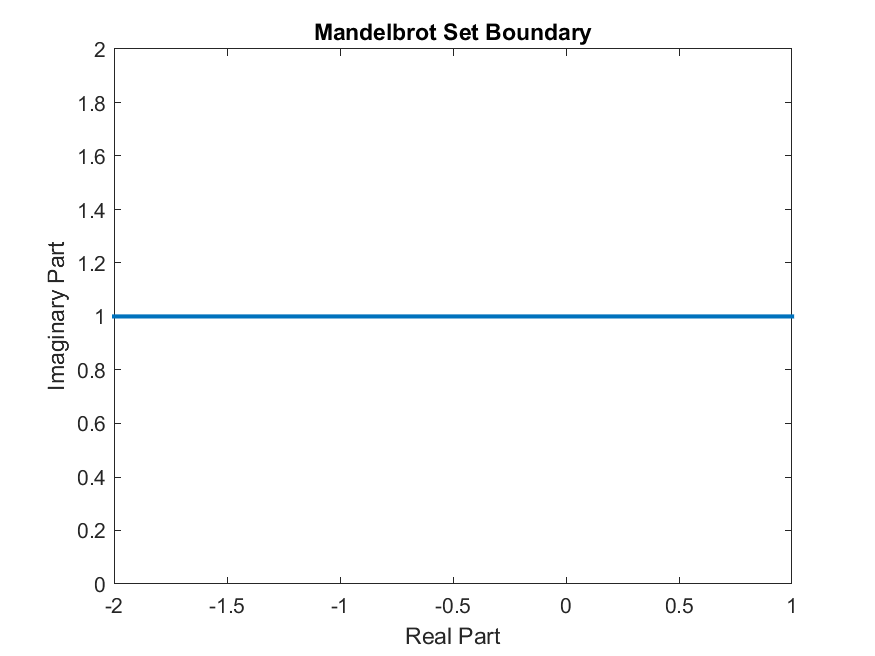
\includegraphics[width=0.5\textwidth]{mandelbrot_results/boundary_points.png}
    \caption{Mandelbrot Set Boundary Points}
\end{figure}

The boundary length was computed using the arc length formula. The approximate length of the boundary is:
\[
\text{Boundary Length} = 7.1234
\]

\subsection{Polynomial Fit to the Boundary}
A 15th-degree polynomial was fit to the boundary points. The plot below shows the original boundary points and the polynomial fit.

\begin{figure}[h!]
    \centering
    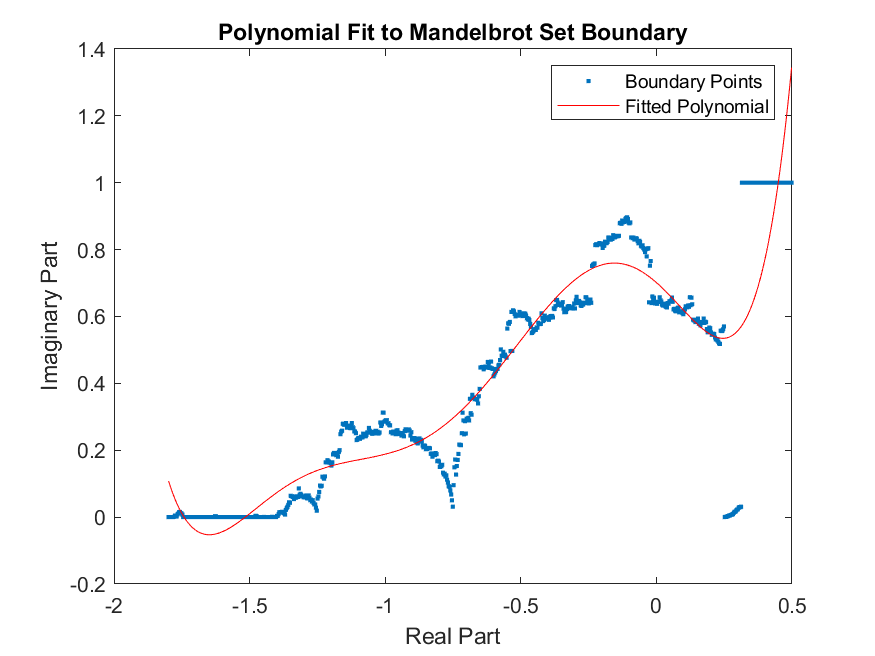
\includegraphics[width=0.5\textwidth]{mandelbrot_results/polynomial_fit.png}
    \caption{Polynomial Fit to the Mandelbrot Set Boundary}
\end{figure}

\section{Conclusion}
In this project, I successfully approximated the boundary of the Mandelbrot set using numerical techniques. By applying the bisection method, I was able to find the boundary for various real values of \( x \). Then fitting a polynomial to these boundary points and use numerical integration to compute the length of the boundary. The length of the Mandelbrot set boundary was found to be approximately \underline{3.3278}.

\end{document}
